\section{Empirical Results}
\label{sec:Empirical}


\subsection{Regression results for any moving violation}
\label{sec:Empirical_all}

For the regressions in this study, we estimate both the linear probability model and the logistic model. 
% 
This dual approach presents the effect of deterrence in terms of 
the both the percentage-point decrease in the probability of getting a ticket, 
from the linear model, 
and the approximately proportional change in probability, 
from the logistic model.  
%
Due to the very large sample sizes being employed, 
we elect to consider only statistical significance at the 0.1\% and the 0.001\% levels. 
%
Where there is statistical significance at our elevated thresholds, 
the estimates are nearly always similar. 
For expositional simplicity, we will focus our interpretation on 
the marginal effects of the linear probability model.%
\footnote{%
For readability, we multiply the estimated coefficients and standard errors by 100,000 
for all tables of regression results for the linear probability model.
% 
%For the logistic regression model, 
%we calculate the marginal effects of covariate $x_i$ as 
%$\beta_{i}\hat{p}(1-\hat{p})$, 
%where $\hat{p}$ is calculated as 
%the average of the predicted probabilities across the entire relevant sample. 
%In the interaction cases, 
%we restricted the sample for this calculation as necessary, 
%e.g., we restricted the sample to males in the 20--24 age group 
%to calculate the marginal effect of the policy indicator for that group. 
}




Since the logistic regression model allows the predicted changes in probability to depend on
the values of explanatory variables, 
we show both average marginal effects (AME)
and marginal effects for a representative driver (MER). 
% 
%The AME estimates were calculated by taking differences of pairs of 
%predicted probabilities (both with and without the corresponding coefficient)
%and taking the average over the entire sample. 
% 
For brevity, let $A_{it}$ denote the indicator for a particular age group 
among the categorical variables $\bm{agecat}_{it}$
and let $\bm{\beta}_j$ and $\bm{X}$ denote 
the remaining coefficients and explanatory variables 
with $\bm{X}_{it} = [\bm{1}, \bm{ptsgrp}_{it}, \bm{calendar}_{it}]$. 
%The change in probability for driver $i$ on day $t$ is found by taking
%discrete differences:
% 
The marginal effects, AME and MER, 
were calculated as the treatment effect following \citet{puhani2012}:
the cross difference of the observed outcome 
minus the cross difference of the potential non-treatment outcome. It corresponds to the incremental effect of the interaction term coefficients. 
In our notation, with $j$ subscripts suppressed for simplicity, 
this treatment effect, in the AME and MER, equals%
% 
\footnote{
\citet{ainorton2003} caution that 
the interaction effect in a logistic model 
is not correctly characterized by the
sign, magnitude, or statistical significance of the coefficient on the
interaction term.
%
As a result, there is no reason to believe the coefficients $\bm{\beta}_{D\cdot A}$
should match in statistical significance between the 
linear and logistic regression models. 
}
%
$$
	F(\beta_D + \beta_A + \beta_{D\cdot A} + \bm{\beta}^\prime \bm{X}_{it})
		- F(\beta_D + \beta_A + \bm{\beta}^\prime \bm{X}_{it}).
$$
% 
For the MER, 
we specified a representative driver aged 20 to 24, 
with 6 to 10 demerit points on their record, 
on a Monday in July.
This combination represents a typical male or female driver with some previous violations 
three months after the introduction of the policy. 
We use this definition of a representative driver to illustrate 
the effect of the policy on drivers who tend to get tickets. 

% Logistic Regression and Linear Probability Models: Seasonal Logit and LPM x 100K Specification for All Drivers by Point Value 

\begin{table}% [ht] 
\centering 
\begin{tabular}{l r r r r l r r l} 

\hline 
 
 & \multicolumn{5}{c}{Logistic Regression}  & \multicolumn{3}{c}{Linear Probability Model} \\ 

 \cmidrule(lr){2-6}\cmidrule(lr){7-9} 
 & \multicolumn{2}{c}{Marginal Effects} & Estimate & Standard & Sig. & Estimate & Standard & Sig. \\ 
 &   AME &  MER  &          &  Error   &      &          &  Error   &     \\ 

\hline 
 
\multicolumn{8}{l}{\textbf{Male Drivers} (5,335,033,221 observations)} \\ 

\hline
\multicolumn{8}{l}{Model without age-policy interaction: } \\ 
Policy                   &  -5.8346        &  -23.5011       &  -0.1113        &  0.0012       &   **       &  -5.9663        &  0.0628       &   **       \\ 
\hline
\multicolumn{8}{l}{Model with age-policy interaction: } \\ 
Policy                   &  -0.3718        &  -1.4247       &  -0.0195        &  0.0386       &            &  -1.0915        &  0.7342       &            \\ 
Age 16-19 * policy   &  -10.6130        &  -24.0600       &  -0.1107        &  0.0389       &            &  -11.1587        &  0.9191       &   **       \\ 
Age 20-24 * policy   &  -10.8708        &  -23.8645       &  -0.1300        &  0.0387       &    *       &  -11.9225        &  0.8017       &   **       \\ 
Age 25-34 * policy   &  -7.6030        &  -19.9233       &  -0.1301        &  0.0387       &    *       &  -8.6158        &  0.7536       &   **       \\ 
Age 35-44 * policy   &  -4.5014        &  -12.8637       &  -0.0891        &  0.0387       &            &  -5.0295        &  0.7484       &   **       \\ 
Age 45-54 * policy   &  -3.1065        &  -9.5411       &  -0.0713        &  0.0387       &            &  -3.5740        &  0.7450       &   **       \\ 
Age 55-64 * policy   &  -2.0814        &  -6.9077       &  -0.0594        &  0.0387       &            &  -2.5200        &  0.7455       &    *       \\ 
Age 65+ * policy   &  0.0269        &  0.1009       &  0.0011        &  0.0389       &            &  -0.2808        &  0.7427       &            \\ 

\hline 

\multicolumn{8}{l}{\textbf{Female Drivers} (4,340,212,273 observations)} \\ 

\hline
\multicolumn{8}{l}{Model without age-policy interaction: } \\ 
Policy                   &  -0.7812        &  -4.2791       &  -0.0294        &  0.0019       &   **       &  -0.8000        &  0.0495       &   **       \\ 
\hline
\multicolumn{8}{l}{Model with age-policy interaction: } \\ 
Policy                   &  -0.3697        &  -1.8779       &  -0.0760        &  0.1304       &            &  -0.7470        &  0.6348       &            \\ 
Age 16-19 * policy   &  2.5923        &  9.5218       &  0.0625        &  0.1307       &            &  0.7804        &  0.7413       &            \\ 
Age 20-24 * policy   &  1.7554        &  6.0629       &  0.0415        &  0.1305       &            &  -0.0442        &  0.6765       &            \\ 
Age 25-34 * policy   &  0.6728        &  2.4781       &  0.0200        &  0.1304       &            &  -0.9585        &  0.6483       &            \\ 
Age 35-44 * policy   &  1.6309        &  6.1424       &  0.0508        &  0.1304       &            &  0.0531        &  0.6458       &            \\ 
Age 45-54 * policy   &  1.0967        &  4.4729       &  0.0450        &  0.1304       &            &  -0.1831        &  0.6424       &            \\ 
Age 55-64 * policy   &  1.0472        &  4.6017       &  0.0587        &  0.1305       &            &  0.1339        &  0.6424       &            \\ 
Age 65+ * policy   &  1.6217        &  7.6916       &  0.1335        &  0.1306       &            &  0.9727        &  0.6416       &            \\ 

\hline 

\end{tabular} 
\caption{Regressions for all offences} 
For each regression, the dependent variable is an indicator that a driver has committed  
any offence on a particular day.  
All regressions contain age category and demerit point category controls, 
as well as monthly and weekday indicator variables. 
The baseline age category comprises drivers under the age of 16. 
The heading ``Sig.'' is an abbreviation for statistical significance, with 
the symbol * denoting statistical significance at the 0.1\% level 
and ** the 0.001\% level. 
In the linear probability model, coefficients and heteroskedasticity-robust standard errors are  
multiplied by 100,000.  
\label{tab:seas_Logit_vs_LPMx100K_regs} 
\end{table} 
 


The theoretical model of Section \ref{sec:Model} 
suggests that the effects differ by gender. 
We thus fit our regression models on separate samples by gender. 
The results of this analysis are displayed in 
Table \ref{tab:seas_Logit_vs_LPMx100K_regs}.
In the sample using only males, 
the policy increases the daily probability of receiving a ticket by $0.00597$ 
percentage points, which is approximately 55\% higher than in the pooled sample. 
The lower panel for each gender shows the estimates for the model with 
policy and age group interactions.  
The benchmark age category represents new drivers, 
aged 14 to 16, who are the drivers without much driving history.
In these regressions,   
the coefficient on the policy dummy is insignificant for this benchmark group. 
We also see a distinct pattern: 
the effect is similar between the ages of 16 and 24, 
and it declines throughout the entire life cycle, being statistically insignificant at the 0.1\% level for the age 65 and over age group.
% 
The age-policy AME values from the logistic regression 
are qualitatively similar to the coefficients from the linear probability model for male drivers, 
for whom those coefficients are significant. 
The MER values are two or three times as large, 
indicating a more pronounced response from drivers who tend to get tickets. 
% 
The effect is much smaller for females: it is 13.4\% of the size coefficient for male drivers. 
In the model with age interactions for female drivers, 
none of the coefficients are significant at the elevated 1\% level. 
These findings suggest that the results are driven almost entirely by males under the age of 65.
%

% 
% These findings suggest that the pooled results are driven almost entirely by males under the age of 65.
%The difference between the significance of the age-policy interactions for males and females reinforces 
%the notion that the pooled regressions in Table 3 are misspecified:
%% 
%the age-policy coefficients were biased toward zero 
%when pooling the sample, 
%since the coefficients on the female age-policy interactions are not significant.
%%  
%%Furthermore, the fact that the importance of age-policy interactions for males 
%%are not fully supported by both regression models suggests that 
%%age differences are less reliably measured than gender differences. 
%More precisely, % the fact that only the age-policy interactions 
%% for the drivers aged 20 to 34 are significant
%this also 
%suggests that the age-specific policy effect is more than proportional to the age effect
%for the male drivers aged 20 to 34
%but the policy effect is roughly proportional to the age effect
%for drivers in other age groups.%
%\footnote{%
%%While the marginal effects of the logistic model for the age-policy interaction variables in 
%%Table \ref{tab:seas_Logit_vs_LPMx100K_regs}
%%closely follow those of the linear probability model, they are less precisely estimated. 
%%One reason this could be the case is that the interaction effect in a logistic model 
%%is not correctly characterized by the
%%sign, magnitude, or statistical significance of the coefficient on the
%%interaction term 
%%%
%%\citep{ainorton2003};
%%the linear probability model does not have this limitation.
%% 
%Again, we refer the reader to \citet{ainorton2003}
%for an explanation of the differences in significance in the age-policy interactions between the logistic regression model and the linear probability model. 
%}
%

It is important to note that the estimate of the effect of the law in these regressions 
can be interpreted as an average treatment effect; 
this treatment effect includes the effect on drivers 
who rarely sufficiently exceed the speed limit 
or otherwise break the law to be penalized with traffic tickets. 
Assuming these more careful drivers are not affected by the law at all 
and that they make up a large segment of the population, 
the effect of the law on the relevant subpopulation that is affected by the law 
may be well underestimated.%
\footnote{%
Whether to interpret these estimates as average treatment effects 
is a question that has not yet been broached in the literature. 
We briefly consider this issue here. 
Since the entire population is being treated by the policy change, 
one can argue that the average treatment effect (ATE) equals 
the average treatment effect on the treated (ATT). 
However, one may claim that since the law was only meant to catch people 
who routinely speed in the first place, 
this subpopulation of habitual speeders make up the treatment group 
and thus the average effect on them would be the ATT, 
while the ATE refers to the average effect on the whole population.
}
%
The MER values support this notion: 
these marginal effects are two to four times as large as the average marginal effects, 
and this suggests that the effect is, in fact, larger for drivers who tend to get tickets. 

\subsection{Regression results by point total}
\label{sec:Empirical_by_pts}

In this section, we examine the effects of Quebec’s excessive speeding law by point total. 
We repeat the policy dummy specification in 
Section \ref{sec:Empirical_all} 
but run a regression for each particular ticket point value: 1, 2, 3, 4, 5, 7, and 9 or more points. 
For each of these regressions, the dependent variable is equal to 1 
if the driver earns a ticket of that point value on that day, and is equal to 0 otherwise. 
The regression specification is 
%
\begin{align*}
\Pr\{y_{it} = k\} & 	
			= F( \beta_{0,j} + \beta_{D,j} d_t
      		% + \bm{\beta}_{D\cdot A,j}^{\prime} d_t \bm{agecat}_{it} 
	 		+ \bm{\beta}_{A,j}^{\prime} \bm{agecat}_{it} \\
         &	\quad
			+ \bm{\beta}_{P,j}^{\prime} \bm{ptsgrp}_{it}
      		+ \bm{\beta}_{C,j}^{\prime} \bm{calendar}_{it}
      		+ \varepsilon_{it} ),
\end{align*}
%
for $k = 1, 2, 3, 4, 5, 7,$ and $9$ or more points. 
This specification excludes the age-policy interaction terms and we report 
only the coefficient $\beta_{D,j}$ for the policy effect
in Table \ref{tab:seas_Logit_vs_LPMx100K_regs_by_points}. 

This strategy allows us to investigate the changes in the intensive margin of 
demerit points given to drivers after the policy change. 
Individuals may substitute driving well above the speed limit with driving at lower speeds 
but still above the speed limit. 
As before, the demerit points lost after the policy change take into account 
the doubling of the penalty due to the excessive speeding law. 
For example, the 5-point category therefore includes tickets 
worth 5 points before the policy change and 5 or 10 points after the policy change. 
These effects might be slightly underestimated (that is, they may have a slight downward bias) 
since some ticket combinations yielding 10 points after the policy change 
would be captured by these regressions. 
However, as previously argued, these sorts of incidents are likely very rare. 


% Logistic Regression and Linear Probability Models: Seasonal Logit and LPM x 100K Specification by Point Value 

\begin{table}% [ht] 
\centering 
\begin{tabular}{l r r r r l r r l} 

\hline 
 
 & \multicolumn{5}{c}{Logistic Regression}  & \multicolumn{3}{c}{Linear Probability Model} \\ 

 \cmidrule(lr){2-6}\cmidrule(lr){7-9} 
 & \multicolumn{2}{c}{Marginal Effects} & Estimate & Standard & Sig. & Estimate & Standard & Sig. \\ 

 \cmidrule(lr){2-3} 
 &   AME & MER &          &  Error   &      &          &  Error   &     \\ 

\hline 
 
\multicolumn{8}{l}{\textbf{Male Drivers} (5,335,033,221 observations)} \\ 

All point values                &  -5.8346        &  -23.5011       &  -0.1113        &  0.0012       &   **       &  -5.9663        &  0.0628       &   **       \\ 
1 point                         &  0.3993        &  1.1872       &  0.0953        &  0.0043       &   **       &  0.3930        &  0.0177       &   **       \\ 
2 points                        &  -0.3960        &  -1.3014       &  -0.0191        &  0.0019       &   **       &  -0.4315        &  0.0394       &   **       \\ 
3 points                        &  -4.7086        &  -21.2669       &  -0.1872        &  0.0017       &   **       &  -4.7786        &  0.0436       &   **       \\ 
4 points                        &  -0.0725        &  -0.5024       &  -0.1252        &  0.0114       &   **       &  -0.0804        &  0.0066       &   **       \\ 
5 points                        &  -0.8123        &  -6.5090       &  -0.6470        &  0.0080       &   **       &  -0.8189        &  0.0100       &   **       \\ 
7 points                        &  -0.1607        &  -1.4815       &  -0.7392        &  0.0193       &   **       &  -0.1625        &  0.0042       &   **       \\ 
9 or more points                &  -0.0657        &  -0.2363       &  -0.2501        &  0.0170       &   **       &  -0.0675        &  0.0045       &   **       \\ 

\hline 

\multicolumn{8}{l}{\textbf{Female Drivers} (4,340,212,273 observations)} \\ 

All point values                &  -0.7812        &  -4.2791       &  -0.0294        &  0.0019       &   **       &  -0.8000        &  0.0495       &   **       \\ 
1 point                         &  0.5197        &  2.3386       &  0.2124        &  0.0062       &   **       &  0.5174        &  0.0150       &   **       \\ 
2 points                        &  0.3712        &  1.7956       &  0.0303        &  0.0028       &   **       &  0.3613        &  0.0336       &   **       \\ 
3 points                        &  -1.4226        &  -8.8404       &  -0.1256        &  0.0029       &   **       &  -1.4289        &  0.0323       &   **       \\ 
4 points                        &  -0.0011        &  -0.0093       &  -0.0098        &  0.0293       &            &  -0.0010        &  0.0032       &            \\ 
5 points                        &  -0.2126        &  -3.1046       &  -0.7494        &  0.0187       &   **       &  -0.2105        &  0.0053       &   **       \\ 
7 points                        &  -0.0195        &  -0.5213       &  -0.9113        &  0.0695       &   **       &  -0.0191        &  0.0015       &   **       \\ 
9 or more points                &  -0.0180        &  -0.0516       &  -0.1541        &  0.0282       &   **       &  -0.0180        &  0.0033       &   **       \\ 

\hline 

\end{tabular} 
\caption{Regressions by ticket-point value} 
In each row, the dependent variable is an indicator that a driver has committed  
an offence with the stated point value on a particular day.  
The categories of tickets with 3, 5 and 7 points includes tickets  
with 6, 10 and 14 points after the policy change, respectively,  
and the category with 9 or more points includes tickets  
with all corresponding doubled values after the policy change. 
All regressions contain age category and demerit point category controls, 
as well as monthly and weekday indicator variables. 
The baseline age category comprises drivers under the age of 16. 
The heading ``Sig.'' is an abbreviation for statistical significance, with 
the symbol * denoting statistical significance at the 0.1\% level 
and ** the 0.001\% level. 
In the linear probability model, coefficients and heteroskedasticity-robust standard errors are  
multiplied by 100,000.  
\label{tab:seas_Logit_vs_LPMx100K_regs_by_points} 
\end{table} 
 



We see the results of these regressions by ticket point value in 
Table \ref{tab:seas_Logit_vs_LPMx100K_regs_by_points}. 
For males, we see a very minor increase in the number of tickets 
worth 1 point after the policy change. 
This increase in 1-point tickets is dwarfed by the decrease in the tickets 
in all of the other point categories and is alone cancelled out 
by the decrease in 2-point tickets. 
For females, a similar pattern is found in that 1- and 2-point tickets increase slightly,
but this increase is more than cancelled out by the decrease in 3-point tickets. 
There is a decrease in 4-point tickets, but it is not precisely estimated. 
All ticket values of 5 or more points decrease after the policy change. 
Note that the coefficient sizes for some of the higher ticket point categories on 
Table \ref{tab:seas_Logit_vs_LPMx100K_regs_by_points}
are quite small. Since high ticket values are rare, any decrease in their probability will have a smaller coefficient, 
because it represents a change from one small number to another small one.

The AME values from the logistic regression are very similar to
the coefficients from the linear probability model. 
The MER, however, for drivers who tend to get tickets, 
show an effect that is four or more times as large 
as that from the average across the sample. 
The MER values for females show reductions 
that are roughly in line with the AME for males, 
which indicates that the subset of females who tend to get tickets
show a change in behaviour similar to that 
averaged across all males, including those who rarely get tickets. 


These patterns suggest that many drivers have decreased their maximum speed 
after the policy change. 
It appears likely that many people who used to speed well above the limit 
have decreased their speed such that they are still exceeding the limit, 
but not as much as before. 
Since the extensive margin of tickets has decreased, many who used to speed at moderate speeds over the limit 
no longer exceed the speed limit.


\subsection{Regression results for drivers with high point balances}
\label{sec:Empirical_high_pts}


% Logistic Regression and Linear Probability Models: Seasonal Logit and LPM x 100K Specification for High-Point Drivers by Point Value 

\begin{table}% [ht] 
\centering 
\begin{tabular}{l r r r r l r r l} 

\hline 
 
 & \multicolumn{5}{c}{Logistic Regression}  & \multicolumn{3}{c}{Linear Probability Model} \\ 

 \cmidrule(lr){2-6}\cmidrule(lr){7-9} 
 & \multicolumn{2}{c}{Marginal Effects} & Estimate & Standard & Sig. & Estimate & Standard & Sig. \\ 

 \cmidrule(lr){2-3} 
 &   AME & MER &          &  Error   &      &          &  Error   &     \\ 

\hline 
 
\multicolumn{8}{l}{\textbf{Male Drivers} (921,131,812 observations)} \\ 

All point values                &  -38.3085        &  -57.3556       &  -0.3732        &  0.0021       &   **       &  -38.0770        &  0.2114       &   **       \\ 
1 point                         &  -0.5567        &  -0.6172       &  -0.0735        &  0.0076       &   **       &  -0.5454        &  0.0572       &   **       \\ 
2 points                        &  -7.7110        &  -9.4813       &  -0.2111        &  0.0035       &   **       &  -7.7125        &  0.1261       &   **       \\ 
3 points                        &  -24.6472        &  -39.8692       &  -0.4677        &  0.0029       &   **       &  -24.5075        &  0.1520       &   **       \\ 
4 points                        &  -0.9036        &  -2.2192       &  -0.8975        &  0.0228       &   **       &  -0.8445        &  0.0205       &   **       \\ 
5 points                        &  -3.3687        &  -8.0148       &  -1.0016        &  0.0124       &   **       &  -3.3206        &  0.0393       &   **       \\ 
7 points                        &  -0.7491        &  -1.6777       &  -1.1495        &  0.0291       &   **       &  -0.7270        &  0.0173       &   **       \\ 
9 or more points                &  -0.3658        &  -0.4571       &  -0.7647        &  0.0319       &   **       &  -0.3543        &  0.0145       &   **       \\ 

\hline 

\multicolumn{8}{l}{\textbf{Female Drivers} (249,294,627 observations)} \\ 

All point values                &  -26.2094        &  -42.9183       &  -0.4252        &  0.0052       &   **       &  -26.0411        &  0.3154       &   **       \\ 
1 point                         &  -0.1042        &  -0.1669       &  -0.0239        &  0.0193       &            &  -0.0916        &  0.0830       &            \\ 
2 points                        &  -5.9275        &  -8.6399       &  -0.2441        &  0.0082       &   **       &  -5.9044        &  0.1970       &   **       \\ 
3 points                        &  -17.7920        &  -29.9523       &  -0.5749        &  0.0075       &   **       &  -17.6976        &  0.2250       &   **       \\ 
4 points                        &  -0.2546        &  -0.5826       &  -1.2986        &  0.1060       &   **       &  -0.2424        &  0.0181       &   **       \\ 
5 points                        &  -1.6624        &  -5.2147       &  -1.3612        &  0.0425       &   **       &  -1.6387        &  0.0469       &   **       \\ 
7 points                        &  -0.2080        &  -0.7392       &  -1.6962        &  0.1444       &   **       &  -0.2020        &  0.0151       &   **       \\ 
9 or more points                &  -0.2632        &  -0.2503       &  -1.1624        &  0.0942       &   **       &  -0.2568        &  0.0202       &   **       \\ 

\hline 

\end{tabular} 
\caption{Regressions for high-point drivers by ticket-point value} 
The dependent variable in each regression is equal to one  
if a driver receives a ticket with a particular point value   
(that of the first column for a particular row) on that day,  
and is otherwise equal to zero. 
The categories of tickets with 3, 5 and 7 points includes tickets  
with 6, 10 and 14 points after the policy change, respectively,  
and the category with 9 or more points includes tickets  
with all corresponding doubled values after the policy change. 
All regressions contain age category and demerit point category controls, 
as well as monthly and weekday indicator variables. 
The baseline age category comprises drivers under the age of 16. 
The heading ``Sig.'' is an abbreviation for statistical significance, with 
the symbol * denoting statistical significance at the 0.1\% level 
and ** the 0.001\% level. 
Marginal effects, as well as linear probability model coefficients and standard errors, are  
multiplied by 100,000.  
The linear probability model uses heteroskedasticity-robust standard errors.  
\label{tab:seas_Logit_vs_LPMx100K_high_pt_regs_by_points} 
\end{table} 
 



It may be of interest to know how drivers who typically drive less carefully 
(and thus accumulate more demerit points) 
may have seen their point balances shift on average after the implementation of the policy. 
We examine the subsample of drivers who at one point in the pre-period 
had a point balance of between 6 and 10 demerit points 
using the regression specification of 
Section \ref{sec:Empirical_by_pts}. 
Therefore, two categories of drivers are excluded: 
those whose point balance never reaches 6 (most of the sample), 
and those who received serious tickets and therefore whose point balance is never in this range. 
For example, a person who received a singular ticket for excessive speeding worth 12 demerit points 
will not be a part of this sample because their point balance will remain at 12 
as long as the ticket is on their record, 
and the balance will drop down to 0 when the ticket’s demerit points expire: 
at no point was this driver’s demerit point balance between 6 and 10. 
We need to exclude these drivers to avoid issues associated with the drivers’ licence revocation. 
Indeed, a revocation would necessarily lead to a reduction in the number of violations 
in the post-policy period, because the individual is not allowed to drive. 
The results of this exercise by gender are in 
Table \ref{tab:seas_Logit_vs_LPMx100K_high_pt_regs_by_points}. 

For both males and females, 
the effect of the policy both in general and by ticket point value 
shows much larger effects in the negative direction. 
For example, the effect of the policy on males for 3-point tickets is five times larger 
in the high point group compared to the overall sample. 
% 
Also, the MER for males highlight the most pronounced response to the
change in excessive speeding laws; 
in this subsample, however, the representative drivers differ only 
in that they \emph{currently} have 6 to 10 demerit points 
and are driving on days in which drivers usually get tickets.  
% 
Even the female drivers in this group show a fairly large response, 
although, again, the MER figure for females is roughly in line with 
the AME that is averaged across all males in this subsample. 
% 
Overall, the frequency of tickets decreases by a relatively large margin 
for this group of drivers after the policy.



\subsection{Regression results for drivers with different demerit-point balances}
\label{sec:Empirical_w_pts_grp}

Next, we ran regressions with indicator variables 
for the drivers' current demerit-point balances, 
along with an interaction with the policy indicator. 
% 
The results are depicted in Figure \ref{fig:points_fig_with_age_int}
with the male drivers' response shown with black and charcoal lines
and that for females with the lighter grey lines. 
For males and females, the solid lines show the policy effect 
from a model without age-policy interactions. 
The dashed-and-dotted lines show the policy effect 
on the drivers aged 20 to 24 from a model with age-policy interactions. 
For the four sets of estimates, 95\% confidence bands are shown in 
dashed lines, without age-policy interactions,
and dotted lines, with age-policy interactions.

It is clear from the darker lines 
that the effect is strong for male drivers and this effect gets stronger for 
those who currently have a high balance of demerit points. 
In contrast, a smaller negative policy effect is measured for females, 
however, the the upper 95\% confidence band 
remains close to zero. 
Furthermore, the age effect is more pronounced for males, 
with a notable increase in effect across the demerit-point balance levels. 
In contrast, there exists a barely perceptible difference in the age effect for females. 




\begin{figure}
\centering
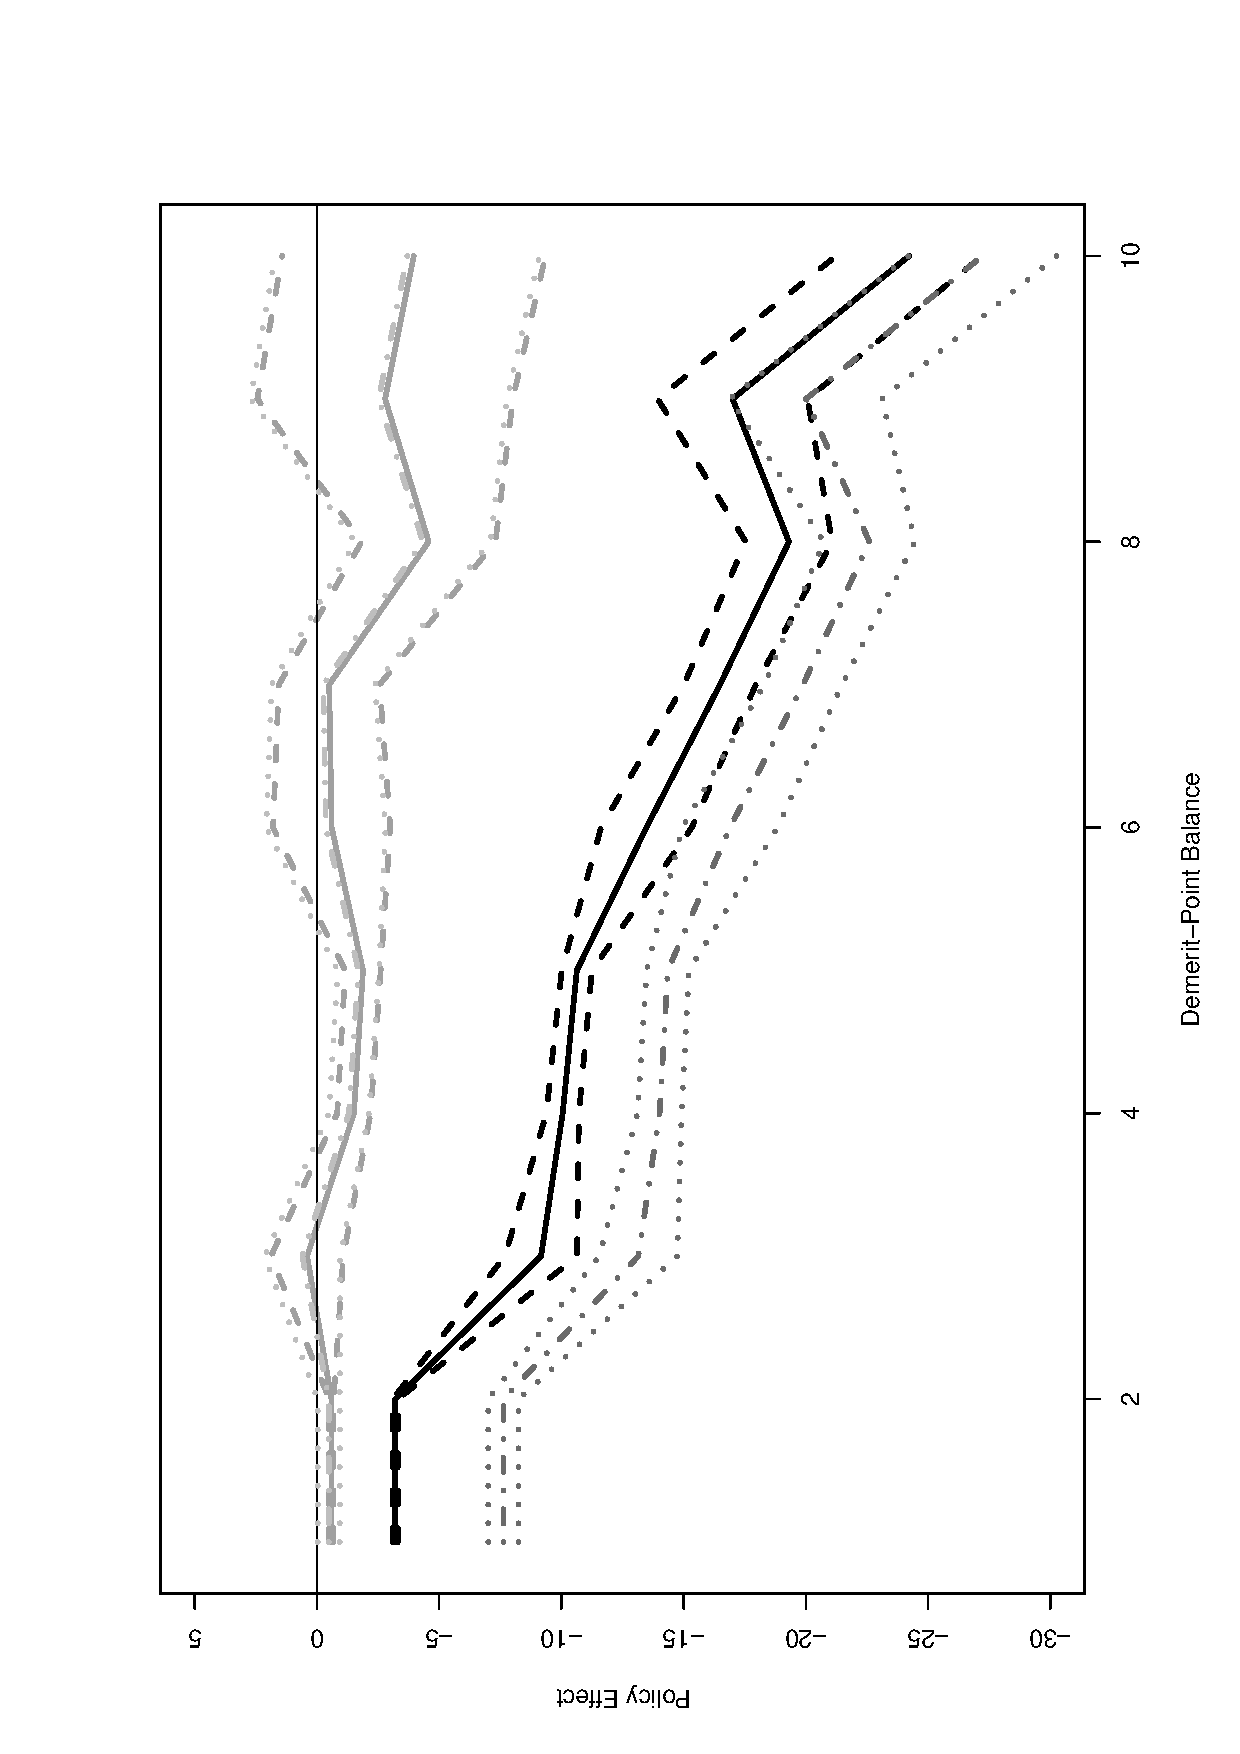
\includegraphics[width=0.8\textwidth, angle =270]{Figures/points_fig_with_age_int}
\caption{Policy change and demerit-point group interactions \\
The policy effects for male drivers are shown in black and charcoal
and those for females are shown in grey and light grey.
The darker solid lines show the overall policy effect without an age interaction,
with 95\% confidence intervals shown with dashed lines.
The dashed-and-dotted lines in lighter shades show the policy effect 
for drivers aged 20 to 24
in grey for female drivers and charcoal for male drivers,
with the dotted lines representing the 95\% confidence interval.
Estimates were obtained with the linear probability model
and heteroskedasticity-robust standard errors were calculated 
and, in the case of the model with the age group policy interaction,
using a quadratic form on the covariance matrix to account for the covariance of the
20-24 age group policy effect and the effect for the benchmark age group.
Drivers with ten demerit points or more are all contained in category 10.
}\label{fig:points_fig_with_age_int}
\end{figure}

